\chapter{Chapter}
\section{Introduction}
Additive manufacturing (AM) is a generic term used to describe the technologies that fabricate 3d Objects directly from 3D model data \cite{KRUTH}. ASTM International defines Additive Manufacturing as the process of joining materials to make objects from 3D model data, usually layer upon layer, as opposed to subtractive manufacturing methodologies \cite{cwig} . 3D Printing is one of the technologies encompassed by AM \cite{Conner}.3D Printing is a manufacturing method  wherein materials like plastic, polymer or metal, are deposited on one another in layers to produce a three dimensional object \cite{sdl}.  The prices of the materials used and the cost of the machinery involved in AM is dropping rapidly as well as the better engineered materials allow for high quality builds leading to the application of this technology in various fields. 

\section{3D Printing Process}

3D Printing is a 3-step process (Figure \ref{fig:3DP}) which includes creating a virtual design of the object (either by using designing software or through 3d scanners), slicing the 3d model before it can be printed followed by printing the object, and final step is the finishing process in which the printed object is cleaned up, polished or sanded, painted to complete it as intended.  
\begin{figure}[ht!]
\centering
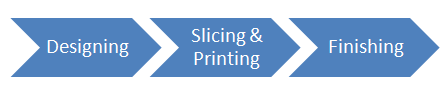
\includegraphics[scale=0.7]{3DPProcess.PNG}
\caption{3-Step 3D Printing Process}
\label{fig:3DP}
\end{figure}

The material chosen to print the object determines the underlying technology for the actual printing process, to name a few, if the material chosen is plastic then Fused Deposition Modeling (FDM) technology is used, for photo sensitive resin material the technology named Photo-polymerization is used, whereas SLS (Selective Laser Sintering) is the technology used if print material is powder (Alumide). Photo-polymerization is a technique that involves the use of UV light to solidify the photosensitive material.  This technique is used by different 3d printing processes like Stereo-lithography (SLA), Digital Light Processing (DLP) and MultiJet printers.  MultiJet printers begin by spraying the tiny droplets of photopolymer in the shape of the first layer followed by cross-linking the polymer by using the UV light from the lamp attached to the print head thus locking the shape of the layer in place \cite{dpW}. Multi-material printers enable fabrication of 3D prints which are composed of diverse materials i.e. materials which are fused to form the object may differ in their chemical properties, and/or physical properties \cite{Doubrovski}.\newline

The step 2 of the 3d Printing process involves the use of a software which enables conversion of the input (i.e. virtual design) to a form which is understood by the print machine. The software fundamentally performs couple of actions enlisted below before the data is sent to the printer:
\begin{itemize}
\item Parses the input and converts it to an internal representation
\item Performs slicing using the internal representation - Slicing is the procedure of dividing the 3D model into 2D layers where in each layer is a \textsl{slice}- a per print layer 2D representation of printer parameters for each (x,y) coordinate. Slicing can be thought of as similar to integrals i.e the 3D object can be approximated by it's derivatives i.e. 2D slices.[see Figure \ref{fig:slicing} \cite{slicing}]
\begin{figure}[ht!]
\centering
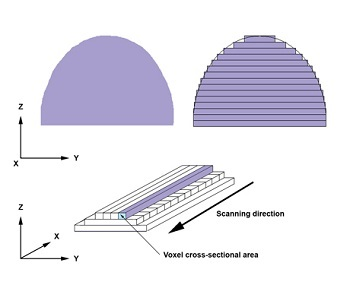
\includegraphics[scale=0.6]{slicing.PNG}
\caption{Slicing}
\label{fig:slicing}
\end{figure}

\item Assign materials to the 2D-Slices. 
\item Convert the 2D slices into machine specific code or representation.
\end{itemize}

The last step of 3D Printing is finishing up the printed object. The importance of this step should not be underestimated as it is worth the enormous effort to make the prints/prototypes look like objects made from real world materials (See Figure\ref{fig:Finishing}). The finishing techniques for the 3D printed objects can be referred as the craftsman's workshop, where patience, skills and experience can help transform the raw products of the printers into fully realized models. Majorly, finishing the prints involves sealing, polishing and painting which helps to bring out the smooth surface and fine feature details. For example, production grade plastic is used by FDM technology to print models which can be sanded, drilled or glued just like any another plastic part. 

\begin{figure}[ht!]
\centering
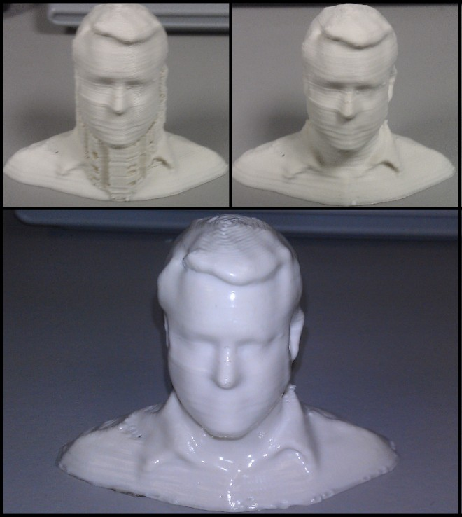
\includegraphics[scale=0.6]{Finishing.png}
\caption{Finishing}
\label{fig:Finishing}
\end{figure}


\section{Problem Statement}

Cuttlefish is a powerful print driver, which performs the transformation of the digital geometric representation of the design into machine-specific code or representation that eventually drives the 3D printer. Cuttlefish supports high-resolution multi-material printers and allows printing large sized multiple objects \cite{cuttlefish}. High-resolution multi-material prints consists of huge amount of voxels(easily up to \begin{math}10^{12}\end{math} as today \textquotesingle s printers allow to combine 7 materials in a single print),a voxel is 3D equivalent of 2D pixel \cite{3DString}. To reproduce the shape and attributes of the 3d model with high precision, Cuttlefish performs material assignment at voxel level. To do so large amount of computational effort is needed which cannot be achieved efficiently by a single processing entity for higher number of objects.  Moreover, cuttlefish processes the input in serial fashion leading to increased amount of computational time for multiple objects. \newline

To achieve a reasonable performance for large computations, distributed computing can be used \cite{DistComp} \cite{Desai}.  Distributed computing is concept where in multiple machines of a distributed system work together on a single problem domain \cite{rouse}.  A distributed system can be defined as the group or cluster of autonomous computers which are connected via network and communicate primarily through message passing \cite{coulouris}. The ultimate goal of distributed computing is to maximize performance by enhancing resource utilization in a cost effective, transparent and reliable manner.\newline

The state of the art multi-jet 3D printers allow printing high resolution large sized multiple print objects at the same time. To efficiently exploit the offered functionality of these printers, appropriate digital fabrication software needs to be developed. Through this master thesis, I have implemented a distributed version of cuttlefish 3dPrinting pipeline by applying the various concepts of distributed computing. The pre-processing task of the large sized multiple objects can be distributed among the nodes of the distributed system so as to utilize the processing power of each node in order to increase the efficiency by limiting the computational effort and time for each node.   Distribution of the tasks among the nodes of the distributed system parallelizes the pre-processing of the input thereby reducing the waiting time for each object to be processed. 